\section{Introduction}
\subsection{Why gpvdm?}
Mankind is facing an existential crisis, by burning fossil fuels we are releasing ~9.795 gigatonnes of $CO_2$ per year, and thus we are steadily changing the composition of Earth's atmosphere. Since 1960, $CO_{2}$ in the atmosphere has risen by around 30\%, this is making our home Earth a more difficult place to live on. As a society we have to reverse this trend if we want to survive. Thin film devices such as solar cells and OLEDs offer a viable way to reduce our $CO_{2}$ emissions, either by providing low carbon electricity, or providing an efficient way to use the energy once generated. It is therefore important that technologies based on thin film devices continue to be developed and succeed. By developing and releasing gpvdm, I hope, I am enabling scientists throughout the world to understand these devices a little bit better, which I hope will contribute in a very small way to solving our climate crisis.



\subsection{Getting more information}
This manual is far from exhaustive please do also watch the \href{https://www.youtube.com/channel/UCbm_0AKX1SpbMMT7jilxFfA}{YouTube} channel where I describe many of the features in more detail. I would suggest you treat the videos as lectures (and take notes) rather than entertaining videos (well I hope they are entertaining too!). New releases are generally announced on \href{https://twitter.com/gpvdm_info}{Twitter}.  I also suggest you also read the papers which were published from this model - do also read the supplementary information (SI) to the papers, as I often write about the model in there.

\subsection{What is the history of gpvdm?}
I started writing gpvdm just after finishing my PhD in 2009 while taking a break for academia and deciding what to do next. At that time it was a simple drift diffusion diode model which did not take account of disorder. The majority of the complex core of gpvdm which deals with disordered materials was written while I was working in the Physics Department at the Imperial College London in 2010-2011. During this time I was working for Jenny Nelson on organic solar cells, it was a very productive and exciting time. Since then the model has been expanded to model many other classes of material system and classes of devices.

\subsection{Bugs}
Firstly thanks for downloading and using gpvdm! I really appreciate this and I hope you find it useful. I get quite a lot of feature requests from people wanting features added or for bugs to be fixed. I really appreciate the feedback!

However, I am currently employed at a UK University and my time is split between teaching, research and admin. My performance in my job is measured by the number of high impact papers I push out per year. I therefore have to prioritize feature requests and bug fixes for people who would like to write a paper with me (i.e. my collaborators).... Therefore if you would like:

\begin{itemize}
  \item A bit of advice on how to do x or y with the model then please do feel free to shoot me a mail, and I will do my best to get back to you. If you don't hear back from me just send the mail again.. I get loads of e-mails, and things get lost if I don't answer quickly.
  \item If you want to report a bug, then please do that, and I will do my best to fix it in the next release. But I can't promise when it will be fixed.
  \item  If you would like a features added or a steady stream of help (i.e. you are asking for my time) then please consider inviting me to join in your work and collaborate on a joint paper. I am happy to add what ever feature you want to the model, or fix what ever bug you may have but in return I would ask for the inclusion of my name on the author list. By doing this it makes it much easier for me to justify sinking time into your project.
\end{itemize}
    
If you don't need help from me to use gpvdm then please feel free to do what you want with the results - no need to contact me.

\pagebreak
\subsection{License}
Gpvdm comprises of three independent components, gpvdm gui, gpvdm core and gpvdm data.  In general everything is under the MIT license except the Python GUI which I have released under GPL v2.0. Details can be found \href{https://github.com/roderickmackenzie/gpvdm/blob/main/LICENSE.md}{here}.

\subsection{Using gpvdm in industrial/academic work}
\label{sec:using_gvpdm}
You are free to use gpvdm in industrial/academic work. In fact, I'm super happy if you use it in your work, papers or books. However, the following further conditions apply:\\\\
1. If you use gpvdm to generate results, then clearly say so in your work. This can be as simple as one sentences saying: "we used gpvdm to perform the simulations" \\\\
2. If you publish a book, paper or thesis where gpvdm has been used you must cite at least three papers associated with the model.  To find out which papers to cite, click on the area indicated in red in figure \ref{fig:cite_me} when using the model.   You are free to choose which papers to cite but PLEASE do not cite the manual. I can't include the manual in paper lists when applying for funding.\\
\\
I ask you to do this because citations are an easy way to demonstrate that people are using gpvdm. Demonstrating use is key to finding money/people to continue the development of gpvdm.  So by doing this you are guaranteeing the future of gpvdm and it's continued availability for others.  Thank you!

\begin{figure}[H]
\centering
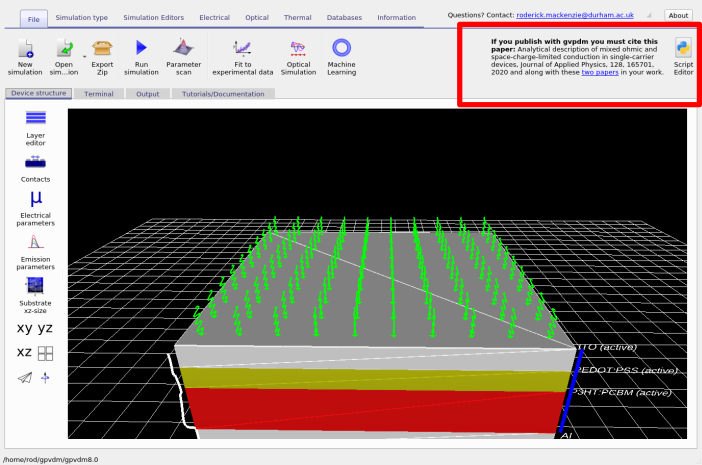
\includegraphics[width=\textwidth]{./images/cite_me2.png}
\caption{If you click on the area indicated by the red box, the model will tell you which papers should be cited.}
\label{fig:cite_me}
\end{figure}



